\documentclass[xcolor=dvipsnames]{beamer}
%\documentclass[handout,xcolor=dvipsnames,pdftex,hyperref={colorlinks=false}]{beamer}

%\usetheme{Boadilla}
\usepackage{appendixnumberbeamer}
\usepackage{amssymb}
\usepackage{amsmath}
\usepackage{subfigure}
\usepackage{hyperref}
\usepackage{url}
\usepackage[english]{babel}
\usepackage{natbib}
\newtheorem{assumption}{Assumption}
\usepackage{helvet}
\usepackage{xcolor}
\usepackage{colortbl}
\usepackage{tikz}
\usepackage{booktabs}
\newcommand{\indep}{{\bot\negthickspace\negthickspace\bot}}

\usepackage{bm}
\newcommand\X{{\bm X}}
%\useoutertheme{infolines}


\usetheme{Warsaw}  % Jens' previous
\usepackage{helvet}
\definecolor{someblue}{rgb}{0,.1,0.8}

\graphicspath{{figures/}{./}}

% == New Commands
% = For general typesetting
\newcommand\spacingset[1]{\renewcommand{\baselinestretch}{#1}\small\normalsize}
\renewcommand\r{\right}
\renewcommand\l{\left}

\newcommand\makegaps{\addtolength{\itemsep}{.25\baselineskip}}
\newcommand\makebiggaps{\addtolength{\itemsep}{.5\baselineskip}}
\newcommand\smallunskip{\vspace{-.25\baselineskip}}
\newcommand\medunskip{\vspace{-.5\baselineskip}}
\newcommand\bigunskip{\vspace{-\baselineskip}}

\newcommand{\VerbBar}{|}
\newcommand{\VERB}{\Verb[commandchars=\\\{\}]}
% Add ',fontsize=\small' for more characters per line
\newcommand{\KeywordTok}[1]{\textcolor[rgb]{0.00,0.44,0.13}{\textbf{{#1}}}}
\newcommand{\DataTypeTok}[1]{\textcolor[rgb]{0.56,0.13,0.00}{{#1}}}
\newcommand{\DecValTok}[1]{\textcolor[rgb]{0.25,0.63,0.44}{{#1}}}
\newcommand{\BaseNTok}[1]{\textcolor[rgb]{0.25,0.63,0.44}{{#1}}}
\newcommand{\FloatTok}[1]{\textcolor[rgb]{0.25,0.63,0.44}{{#1}}}
\newcommand{\CharTok}[1]{\textcolor[rgb]{0.25,0.44,0.63}{{#1}}}
\newcommand{\StringTok}[1]{\textcolor[rgb]{0.25,0.44,0.63}{{#1}}}
\newcommand{\CommentTok}[1]{\textcolor[rgb]{0.38,0.63,0.69}{\textit{{#1}}}}
\newcommand{\OtherTok}[1]{\textcolor[rgb]{0.00,0.44,0.13}{{#1}}}
\newcommand{\AlertTok}[1]{\textcolor[rgb]{1.00,0.00,0.00}{\textbf{{#1}}}}
\newcommand{\FunctionTok}[1]{\textcolor[rgb]{0.02,0.16,0.49}{{#1}}}
\newcommand{\RegionMarkerTok}[1]{{#1}}
\newcommand{\ErrorTok}[1]{\textcolor[rgb]{1.00,0.00,0.00}{\textbf{{#1}}}}
\newcommand{\NormalTok}[1]{{#1}}

\DeclareMathOperator*\plim{plim}
\DeclareMathOperator\rank{rank}
\DeclareMathOperator{\sgn}{sgn}
\def\independenT#1#2{\mathrel{\rlap{$#1#2$}\mkern2mu{#1#2}}}

\title[]{Sensitivity via Omitted Variable Bias}
\subtitle[ ]{PS200C, Spring 2026}
\author[Hazlett]{Chad Hazlett }
\institute[UCLA]{UCLA\\[1ex]
  \texttt{chazlett@ucla.edu}
}
\date{}

\definecolor{dgreen}{rgb}{0,.6,0.8}
\useoutertheme{infolines}

\begin{document}

\subject{Talks}

\begin{frame}
  \titlepage
\end{frame}


%======================================================================
\section{Motivation and example}
%======================================================================

\begin{frame}{Why sensitivity?}
\small
\onslide<1-> Our workflow so far: pick an ID strategy (e.g.\ SOO), defend the assumptions, estimate well.\\
\medskip
\onslide<2-> ``Defend the assumptions'' is the fragile one!\\
\medskip
\onslide<3-> \textbf{Sensitivity analysis}: rather than defending ``confounding $=0$'', ask
\begin{center} \textcolor{Blue}{``How strong would confounding have to be to overturn the conclusion?''} \end{center}
\medskip
\onslide<4-> Old idea --- Cornfield et al.\ (1959) on smoking and lung cancer:\\
\footnotesize
\begin{quote}
\dots an unobserved confounder \dots would need to lead to a nine-fold increase in the odds of smoking to explain away the association \dots and it was asserted that such a strong unobserved confounder was very unlikely to exist.
\end{quote}
\small
\onslide<5-> \textbf{Warning we'll keep repeating}: this is \emph{not} ``how much confounding is there.''
\end{frame}


\begin{frame}{Effects of violence on attitudes: angry or weary?}
\small
\onslide<1-> Among Darfurian refugees in eastern Chad, did exposure to violence make people on average more willing to make concessions to achieve peace (``weary''), or more set on retribution (``angry'')?\\
\medskip
\onslide<2-> \textcolor{Blue}{Central ID claim}: targeting of violence in 2003--2004 was based only on village and gender, otherwise highly indiscriminate. \emph{Being directly harmed is ``as-if random within village$\times$gender strata.''}\\
\medskip
\begin{itemize}
\item<3-> Aerial bombing was extremely crude and difficult to target
\item<4-> \textit{Janjaweed} militia attacks targeted on visible characteristics only (notably $\mathit{female}$)
\item<5-> Purpose was to clear the population, not to pick out rebels
\end{itemize}
\medskip
\onslide<6-> \textcolor{Blue}{Strategy}: SOO conditioning on village and gender.
\end{frame}


\begin{frame}{Darfur: estimate, and the worry}
\small
\onslide<1-> Setup: outcome \textit{PeaceIndex} (0--1); treatment \textit{DirectHarm} (0/1).
\[
\mathit{PeaceIndex}_i = \alpha\,\mathit{DirectHarm}_i + \beta^\top \mathit{Village}_i + \phi\, \mathit{female}_i + \epsilon_i.
\]
\onslide<2-> Those directly harmed are on average \textcolor{Blue}{9.7 percentage points} more pro-peace (SE $=2.3$).\\
\medskip
\onslide<3-> \textbf{But what if the ID strategy is ``a little'' wrong?}\\
\medskip
\onslide<4-> Questions we want sensitivity to help with:
\begin{enumerate}
\item<5-> If somebody names a confounder I don't have, how strong would it have to be to overturn the result?
\item<6-> What about \emph{multiple} confounders, possibly acting non-linearly?
\item<7-> How can we report robustness compactly?
\item<8-> How can we make informed guesses about plausible confounding?
\end{enumerate}
\end{frame}


\begin{frame}{A landscape, and our choice}
\onslide<1-> Several families of sensitivity analysis exist:
\small
\begin{itemize}
\item<2-> \textbf{Matched-pair $\Gamma$ bounds} (Rosenbaum 2002): one odds-of-treatment parameter, for matched designs.
\smallskip
\item<3-> \textbf{Parametric} (Imbens 2003; Carnegie--Dorie--Hill 2016): fully specify a model for $(D, Y, U)$, sweep over its parameters.
\smallskip
\item<4-> \textbf{Partial identification} (Manski 1990; monotonicity bounds): assume less, get ranges.
\smallskip
\item<5-> \textbf{OVB-based} (Frank 2000; Hosman--Hansen--Holland 2010; \textbf{Cinelli \& Hazlett 2020}): use omitted-variable bias as the engine.
\end{itemize}
\bigskip
\onslide<6-> We focus on OVB-based: scale-free in $R^2$, handles multiple/non-linear confounders, and plugs straight into a regression workflow.
\end{frame}


%======================================================================
\section{FWL and OVB}
%======================================================================

\begin{frame}{A short detour: Frisch--Waugh--Lovell}
\small
\onslide<1-> Suppose we run OLS of $Y$ on $D$ and $\X$:
\[
Y = \hat{\tau}\,D + \X\hat{\beta} + \hat{\epsilon}.
\]
\onslide<2-> The same $\hat{\tau}$ is given by a three-step recipe:
\begin{enumerate}
\item Regress $Y$ on $\X$, take residuals $Y^{\perp \X}$
\item Regress $D$ on $\X$, take residuals $D^{\perp \X}$
\item Regress $Y^{\perp \X}$ on $D^{\perp \X}$
\end{enumerate}
\onslide<3-> In words: \emph{multivariate OLS reduces to univariate OLS, after partialling out $\X$},
\[
\hat{\tau} \;=\; \frac{\text{cov}(D^{\perp \X},\, Y^{\perp \X})}{\text{var}(D^{\perp \X})}.
\]
\onslide<4-> This is the central tool for what follows.
\end{frame}


\begin{frame}{Omitted variable bias: setup}
\small
\onslide<1-> Suppose an investigator wishes to run:
\[
Y = \hat{\tau}\, D + \X \hat{\beta} + \hat{\gamma}\, Z + \hat{\epsilon}_{\text{full}}
\]
\onslide<2-> But $Z$ is unobserved, so they run the \emph{restricted} regression:
\[
Y = \hat{\tau}_{\text{res}}\, D + \X \hat{\beta}_{\text{res}} + \hat{\epsilon}_{\text{res}}
\]
\medskip
\onslide<3-> We ask: \textbf{how would $\hat{\tau}$ change if you could include $Z$?}\\
\medskip
\onslide<4-> Whether the ``full'' regression is wise, or whether its coefficient is the quantity of interest, is a separate question --- here we just compute the consequence of omission.
\end{frame}


\begin{frame}{OVB via FWL: $\widehat{\text{bias}} = \hat{\gamma}\hat{\delta}$}
\small
\onslide<1-> Restating FWL,
\[
\hat{\tau}_{\text{res}} \;=\; \frac{\text{cov}(D^{\perp \X},\, Y^{\perp \X})}{\text{var}(D^{\perp \X})}.
\]
\onslide<2-> Substitute the (true) full model $Y = \hat{\tau} D + \X\hat{\beta} + \hat{\gamma} Z + \hat{\epsilon}_{\text{full}}$:
\[
Y^{\perp \X} = \hat{\tau}\, D^{\perp \X} + \hat{\gamma}\, Z^{\perp \X} + \hat{\epsilon}_{\text{full}}^{\perp \X}.
\]
\onslide<3-> Then:
\[
\hat{\tau}_{\text{res}}
= \hat{\tau} + \hat{\gamma}\, \underbrace{\frac{\text{cov}(D^{\perp \X},\, Z^{\perp \X})}{\text{var}(D^{\perp \X})}}_{=:\;\hat{\delta}}
= \hat{\tau} + \hat{\gamma}\hat{\delta}.
\]
\onslide<4-> $\hat{\delta}$ is the coefficient on $D$ in the auxiliary regression
\[
Z = \hat{\delta} D + \X\hat{\psi} + \hat{\epsilon}_Z.
\]
\onslide<5->
\[
\boxed{\;\widehat{\text{bias}}(\hat{\tau}_{\text{res}}) \;=\; \hat{\gamma}\,\hat{\delta} \;=\; \text{impact}\times\text{imbalance}.}
\]
\end{frame}


\begin{frame}{Consider a confounder}
\small
\onslide<1-> Suppose a colleague says:
\begin{quote}
Those near the center of the village were both more likely to be injured \emph{and} have different attitudes.
\end{quote}
\onslide<2-> For each hypothesized pair $(\hat{\gamma}, \hat{\delta})$, the adjusted estimate is $\hat{\tau} = \hat{\tau}_{\text{res}} - \hat{\gamma}\hat{\delta}$.
\smallskip
\onslide<3->
\begin{figure}
\centering
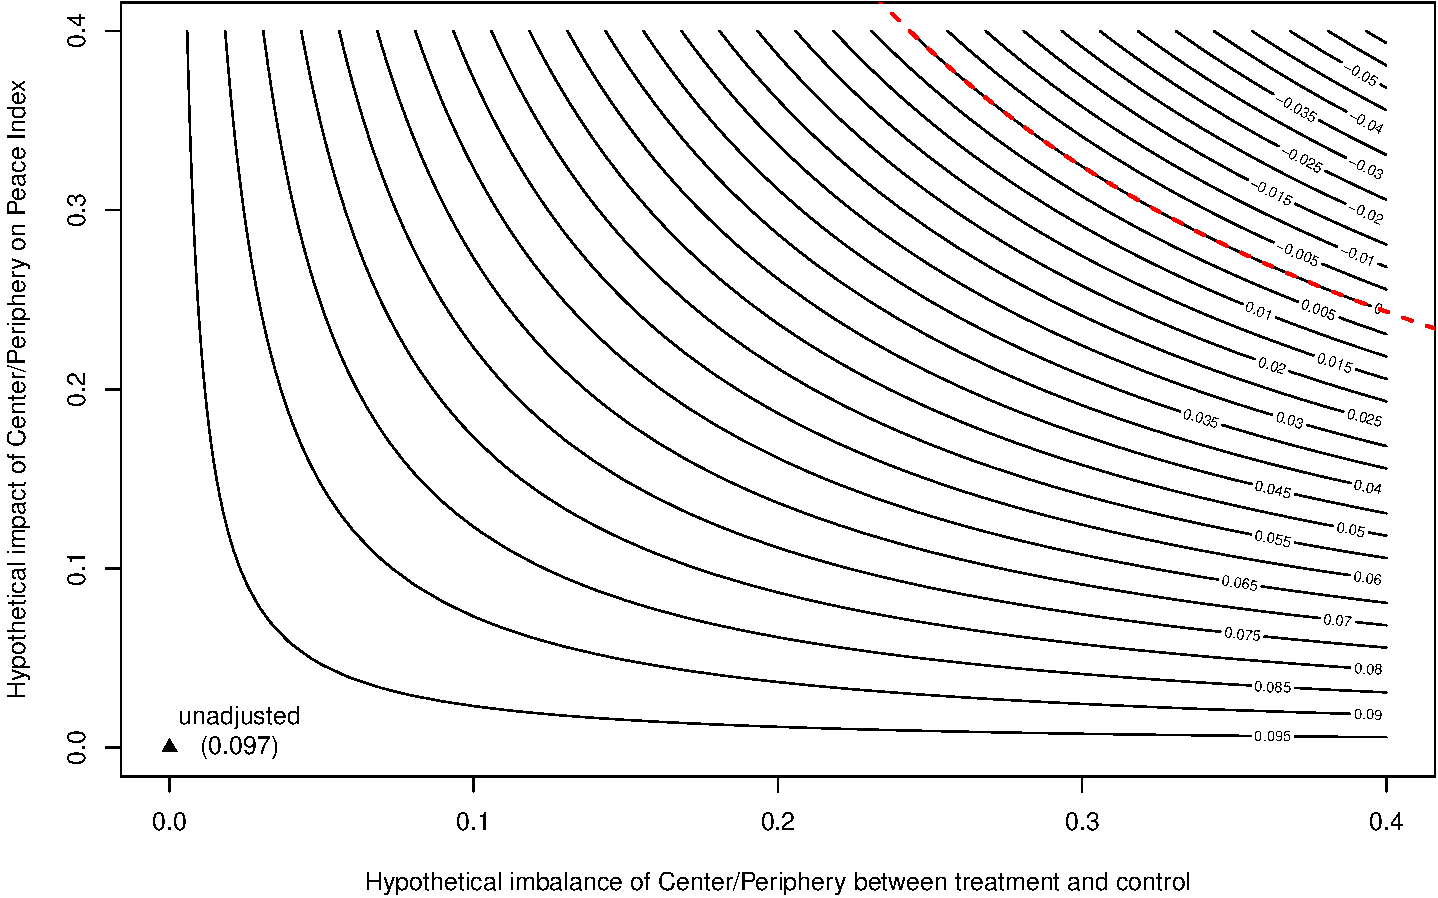
\includegraphics[width=.55\textwidth]{natural_plot_new.pdf}
\end{figure}
\end{frame}


%======================================================================
\section{$R^2$ reparameterization}
%======================================================================

\begin{frame}{Why reparameterize}
\small
\onslide<1-> Problems with the ``natural'' parameterization:
\begin{itemize}
\item<2-> Units of ``impact'' and ``imbalance'' depend on the scale of $Z$. \emph{Center} happened to be binary, but how would you scale a confounder like ``political attitudes''?
\item<3-> ``Name a confounder'' is too narrow. We want to handle multiple confounders, possibly acting non-linearly.
\end{itemize}
\medskip
\onslide<4-> \textbf{Fix:} reparameterize using \emph{partial $R^2$}.
\begin{itemize}
\item<5-> Scale-free, bounded in $[0,1]$
\item<6-> Lets us derive bias \emph{and} variance, do bounds, and handle all confounders jointly.
\end{itemize}
\end{frame}


\begin{frame}{What is the partial $R^2$?}
\small
\onslide<1-> The partial correlation is simply correlation \emph{after} partialling out $\X$:
\[
R_{Y \sim D \mid \X} \;=\; \text{cor}(Y^{\perp \X},\, D^{\perp \X}).
\]
Square it for the partial $R^2$.\\
\medskip
\onslide<2-> Or, ``fraction of variance of $D$ explained by $Z$ beyond what $\X$ explains'':
\[
R^2_{D\sim Z \mid \X} \;=\; \frac{R^2_{D\sim \X + Z} - R^2_{D\sim \X}}{1 - R^2_{D\sim \X}}.
\]
\onslide<3-> And likewise:
\[
R^2_{Y\sim Z \mid D, \X} \;=\; \frac{R^2_{Y\sim D + \X + Z} - R^2_{Y\sim D + \X}}{1 - R^2_{Y\sim D + \X}}.
\]
\onslide<4-> Direction-symmetric: $R^2_{D\sim Z \mid \X} = R^2_{Z \sim D \mid \X}$.
\end{frame}


\begin{frame}{Bias in the $R^2$ parameterization}
\small
\onslide<1-> Take $\widehat{\text{bias}} = \hat{\gamma}\hat{\delta}$, write each coefficient as cov/var via FWL, replace correlations by partial $R^2$'s, and (after some algebra):
\onslide<2->
\[
\boxed{\;|\widehat{\text{bias}}| \;=\; \sqrt{\frac{R^2_{Y\sim Z \mid D, \X}\, R^2_{D\sim Z \mid \X}}{1 - R^2_{D\sim Z \mid \X}}}\;\cdot\; \frac{\text{sd}(Y^{\perp \X, D})}{\text{sd}(D^{\perp \X})}.\;}
\]
\medskip
\onslide<3-> Recall the standard OLS variance fact, $\widehat{\text{se}}(\hat{\tau}_{\text{res}}) = \frac{\text{sd}(Y^{\perp \X, D})}{\text{sd}(D^{\perp \X})\,\sqrt{\text{df}}}$.  So equivalently
\[
|\widehat{\text{bias}}| \;=\; \widehat{\text{se}}(\hat{\tau}_{\text{res}})\,\sqrt{\frac{R^2_{Y\sim Z \mid D, \X}\, R^2_{D\sim Z \mid \X}}{1 - R^2_{D\sim Z \mid \X}}\cdot \text{df}\,}.
\]
\onslide<4-> Everything data-dependent is now in $\widehat{\text{se}}(\hat{\tau}_{\text{res}})$ and df --- both already on your regression printout.
\end{frame}


\begin{frame}{Bias anatomy}
\small
\onslide<1-> Consider the \emph{relative bias} --- the fraction of $\hat{\tau}_{\text{res}}$ that is bias. Using $|\hat{\tau}_{\text{res}}| = |t_D|\,\widehat{\text{se}}(\hat{\tau}_{\text{res}})$,
\[
\frac{|\widehat{\text{bias}}|}{|\hat{\tau}_{\text{res}}|}
\;=\; \frac{\sqrt{\text{df}}\cdot \text{BF}}{|t_D|}
\;=\; \frac{\text{BF}}{|f_{Y\sim D \mid \X}|},
\]
where $\text{BF} := \sqrt{\frac{R^2_{Y\sim Z \mid D,\X}\, R^2_{D\sim Z \mid \X}}{1-R^2_{D\sim Z \mid \X}}}$ is the ``bias factor'' and $f_{Y\sim D \mid \X} := R_{Y\sim D \mid \X}/\sqrt{1 - R^2_{Y\sim D \mid \X}}$ is the partial Cohen's $f$.
\medskip
\onslide<2-> Three things to take away:
\begin{itemize}
\item BF is the expression of confounder strength.
\item $f_{Y\sim D \mid \X}$ --- essentially how much of $Y$'s variance the treatment uniquely explains --- is \emph{all} that enters from the data. It is what confounding is competing to explain.
\item $f_{Y\sim D \mid \X}$ is \emph{not} a function of sample size: more data does not help you fight confounding.
\end{itemize}
\end{frame}


\begin{frame}{Variance anatomy}
\small
\onslide<1-> Applying the same OLS variance fact to the \emph{full} regression and combining:
\[
\widehat{\text{se}}(\hat{\tau}) \;=\; \widehat{\text{se}}(\hat{\tau}_{\text{res}}) \cdot \sqrt{\underbrace{(1-R^2_{Y\sim Z \mid \X, D})}_{\text{VRF}}\,\underbrace{\tfrac{1}{1-R^2_{D\sim Z \mid \X}}}_{\text{VIF}}\,\underbrace{\tfrac{\text{df}}{\text{df}-1}}_{\text{df adj.}}}.
\]
\medskip
\onslide<2->
\begin{itemize}
\item \textbf{VRF}: had we included $Z$, residual $Y$-variance would shrink.
\item \textbf{VIF}: had we included $Z$, its correlation with $D$ would inflate the SE.
\end{itemize}
\end{frame}


%======================================================================
\section{Tools}
%======================================================================

\begin{frame}{First, good to have this in your head}
\begin{figure}
\caption{Contour plot in the partial $R^2$ parameterization}
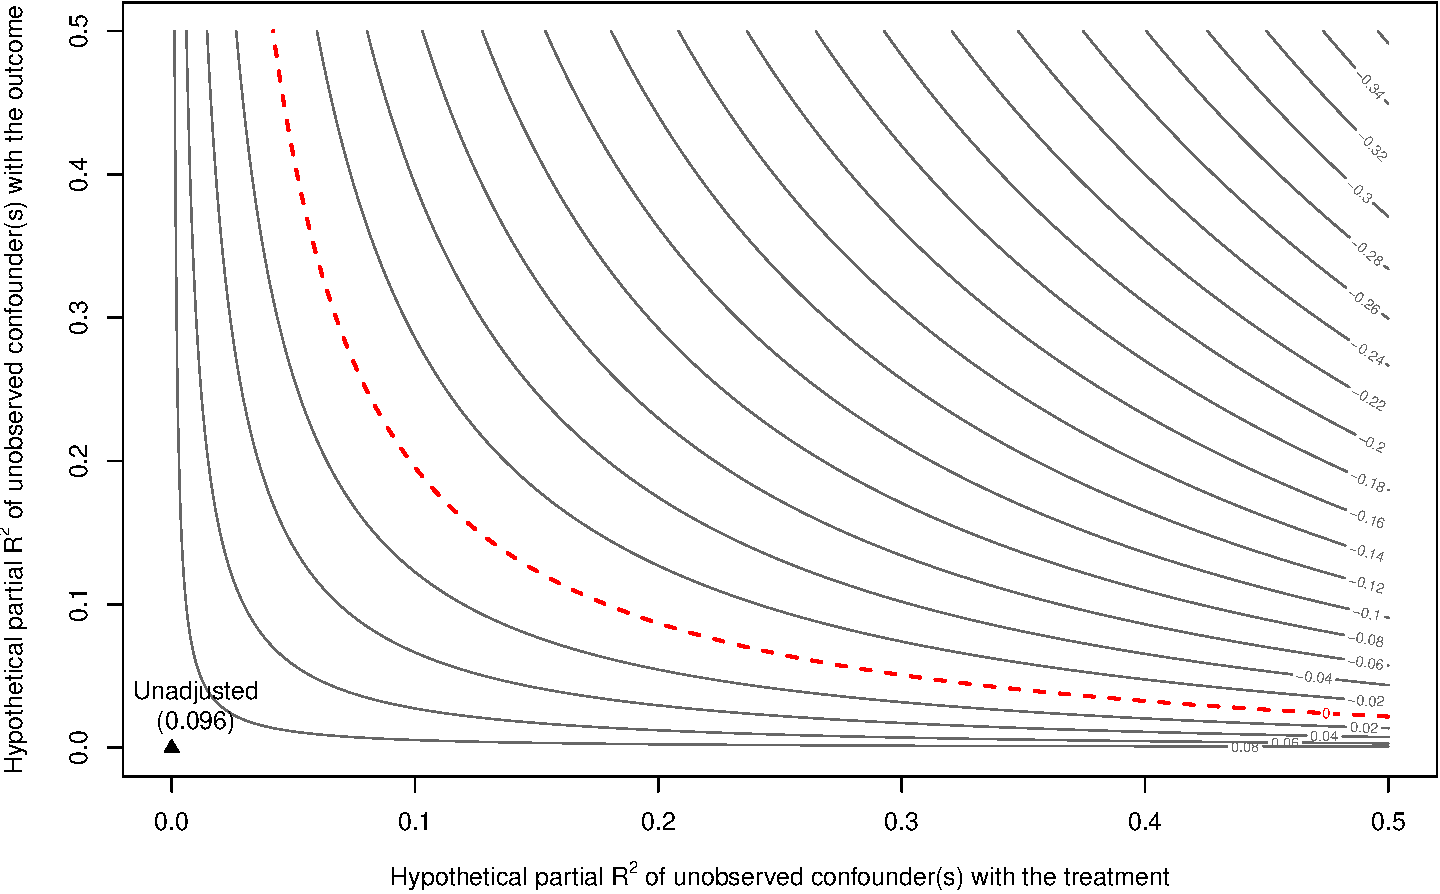
\includegraphics[scale=.4]{contour_nobounds.pdf}
\end{figure}
\end{frame}


\begin{frame}{Two simple statistics for routine reporting}
\small
\onslide<1-> \textbf{Robustness Value (RV)}: the level of (equal) partial-$R^2$ association with $D$ and $Y$ that would eliminate the effect.
\begin{itemize}
\item<2-> $\text{RV}_q$: the equal-association level needed to bring the estimate down by proportion $q$
\item<3-> $\text{RV}_{\alpha}$: the equal-association level needed to bring the $t$-stat to the threshold for level $\alpha$
\end{itemize}
\medskip
\onslide<4-> \textbf{Partial $R^2$ of $D$ with $Y$}: $R^2_{Y\sim D \mid \X}$
\begin{itemize}
\item<5-> If confounding explained \emph{all} residual $Y$-variance, this is how much of $D$ (residual variance) it would have to explain to bring the estimate to zero.
\end{itemize}
\medskip
\onslide<6-> Both come from $t_D$ and df alone --- you can compute them from a published regression table.
\end{frame}


\begin{frame}{Augmented regression table: Darfur}
\footnotesize
\begin{table}[!h] \centering
\begin{tabular}{lrrrrrr}
\multicolumn{7}{c}{Outcome: \textit{Peace Index}} \\
\hline\hline
Treatment:       & Est.  & SE    & $t$    & $R^2_{Y\sim D \mid \X}$ & RV & $\text{RV}_{\alpha=0.05}$ \\
\hline
\textit{Directly Harmed} & 0.097 & 0.023 & 4.18 & 2.2\%  & 13.9\%   &  7.6\%               \\
\hline
$\text{df} = 783$ &       &   \multicolumn{5}{r}{\small \textit{Bound (1$\times$ female):}\ $R^2_y = 12\%$,\ $R^2_d = 1\%$}
\end{tabular}
\end{table}

\onslide<2->
\medskip
Somebody tell us:
\begin{itemize}
\item what does this RV mean?
\item what does this $\text{RV}_{\alpha=0.05}$ mean?
\item what does this $R^2_{Y\sim D \mid \X}$ mean?
\end{itemize}
\end{frame}


% \begin{frame}{Could we benchmark against an observed covariate?}
% \small
% \onslide<1-> Tempting move: ``a confounder \emph{not unlike} an observed $X_j$ would do this much.'' Use $X_j$'s observed partial $R^2$'s with $D$ and $Y$ as a yardstick.\\
% \medskip
% \onslide<2-> But the bias from omitting $Z$ contaminates those very partial $R^2$'s, so naive benchmarking can be misleading.\\
% \medskip
% \onslide<3-> Tiny DGP to illustrate:
% \[
% X = \epsilon_x,\quad Z = \epsilon_z,\quad D = X + Z + \epsilon_d,\quad Y = X + Z + \epsilon_y.
% \]
% \begin{itemize}
% \item<4-> No true effect of $D$ on $Y$.
% \item<4-> $Z$ exactly like $X$ in its relationships to $D$ and to $Y$.
% \item<5-> Honest benchmarking should say: ``a confounder not unlike $X$ would zero the effect.''
% \end{itemize}
% \end{frame}


% \begin{frame}{Informal benchmark vs.\ proper bound}
% \begin{figure}
% 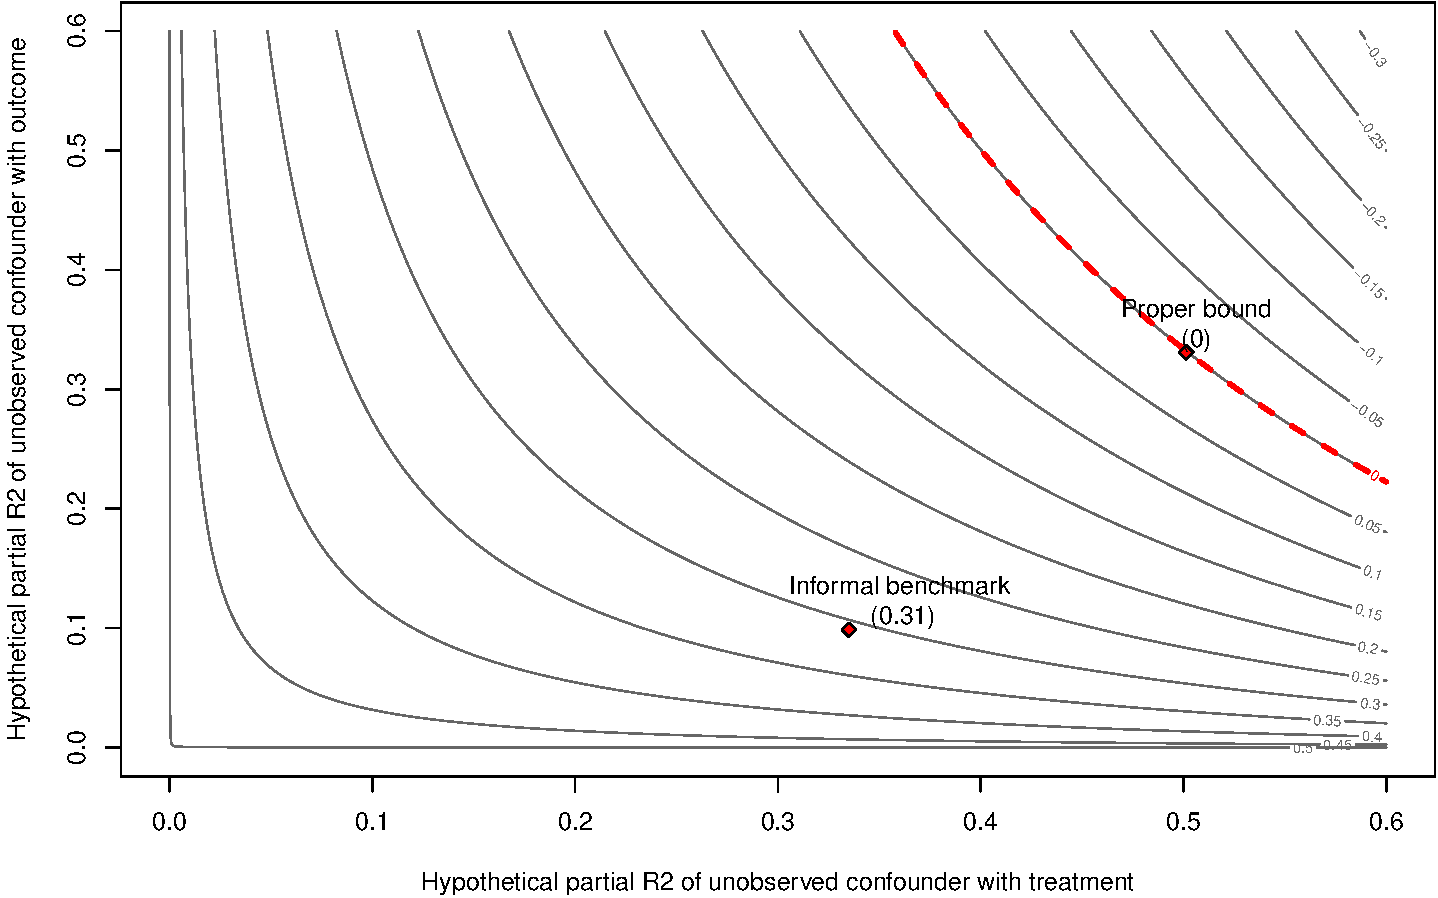
\includegraphics[scale=.48]{informal_vs_bound.pdf}
% \end{figure}
% \footnotesize
% Informal benchmarking (red) understates the bias; the proper bound (blue) gets it right.
% \end{frame}


\begin{frame}{Bounding by comparison to observed covariates}
\small
\onslide<1-> One good interpretational wedge: comparing to an important observed covariate.\\
\medskip
\onslide<2-> For an observed covariate $X_j$, define:\\
\[
k_D := \frac{R^2_{D\sim Z \mid \X_{-j}}}{R^2_{D\sim X_j \mid \X_{-j}}}, \qquad
k_Y := \frac{R^2_{Y\sim Z \mid \X_{-j}, D}}{R^2_{Y\sim X_j \mid \X_{-j}, D}}.
\]
``$Z$ is at most $k_D$ times as predictive of $D$, and $k_Y$ times as predictive of $Y$, as $X_j$ is.''
\medskip
\onslide<2-> Given $\{X_j, k_D, k_Y\}$, this \emph{bounds} both $R^2_{Y\sim Z \mid D,\X}$ and $R^2_{D\sim Z \mid \X}$, and hence the worst-case bias. Conservative for multiple, non-linear confounders. %\footnote{Bound formulas are not as clean as one would hope, because the observed partial $R^2$'s are themselves biased --- see Cinelli \& Hazlett 2020.} 
\medskip
\onslide<3-> \begin{center} \textcolor{Red}{This shows the implications of an assumption --- you still have to argue the assumption itself is believable.} \end{center}
\medskip
\onslide<4-> Example: within Darfur villages, hard to imagine targeting on any basis stronger than $\mathit{female}$. So use $X_j = \mathit{female}$, and vary $k$.
\end{frame}


\begin{frame}{Contour plot with bounds: Darfur}
\begin{figure}
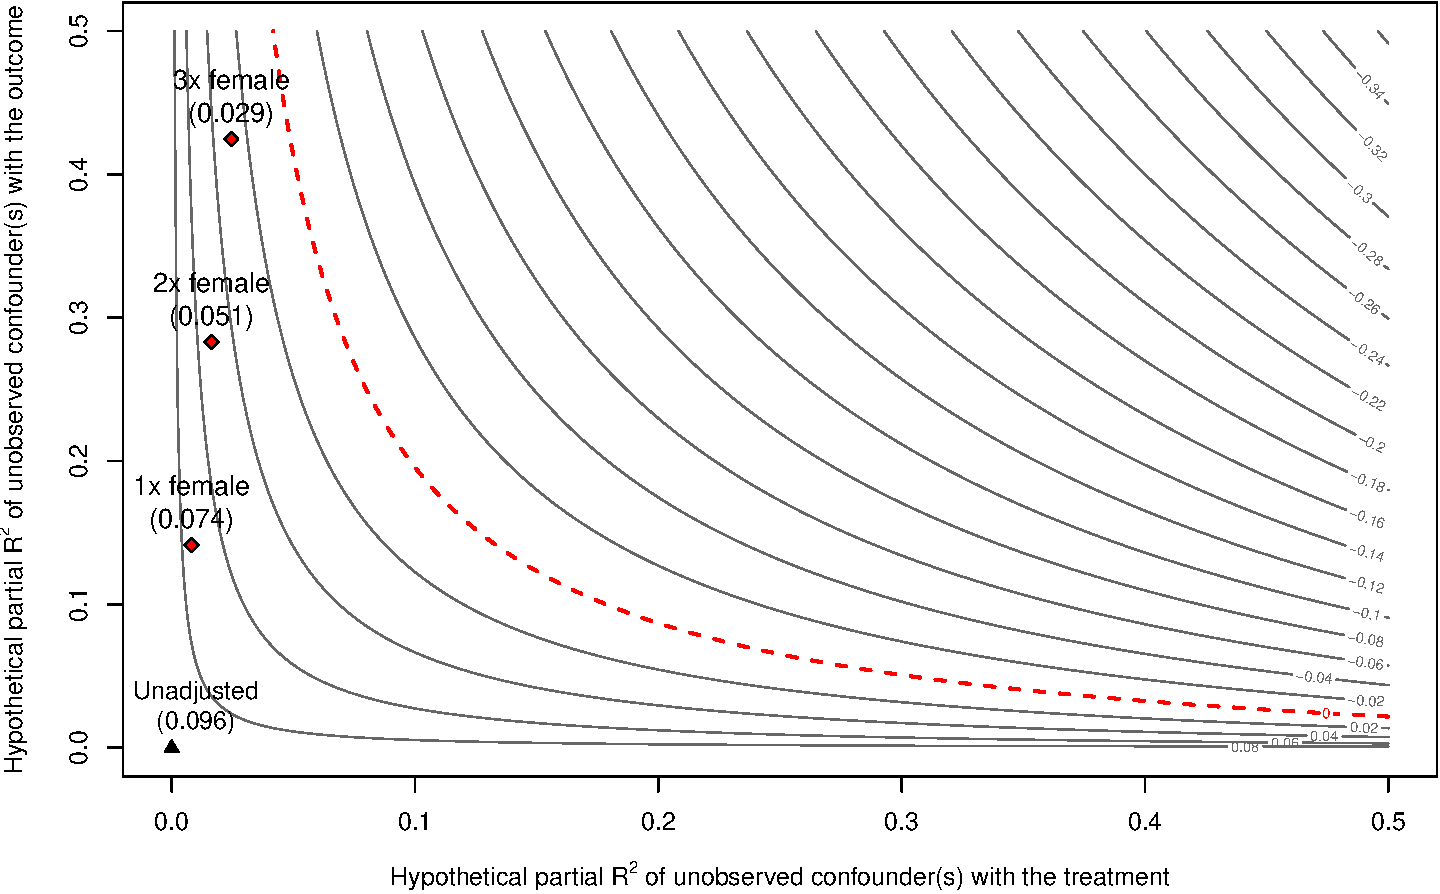
\includegraphics[scale=.45]{r2contour_female.pdf}
\end{figure}
\footnotesize
\vspace{-.2in}
\onslide<2-> Point estimate robust to a confounder $1\times$, $2\times$, or even $3\times$ as strong as $\mathit{female}$.
\end{frame}


\begin{frame}{Inference and extreme scenarios}
\footnotesize
\begin{columns}[T]
\begin{column}{0.5\textwidth}
\centering
\textbf{$t$-statistic contour}\\[2pt]
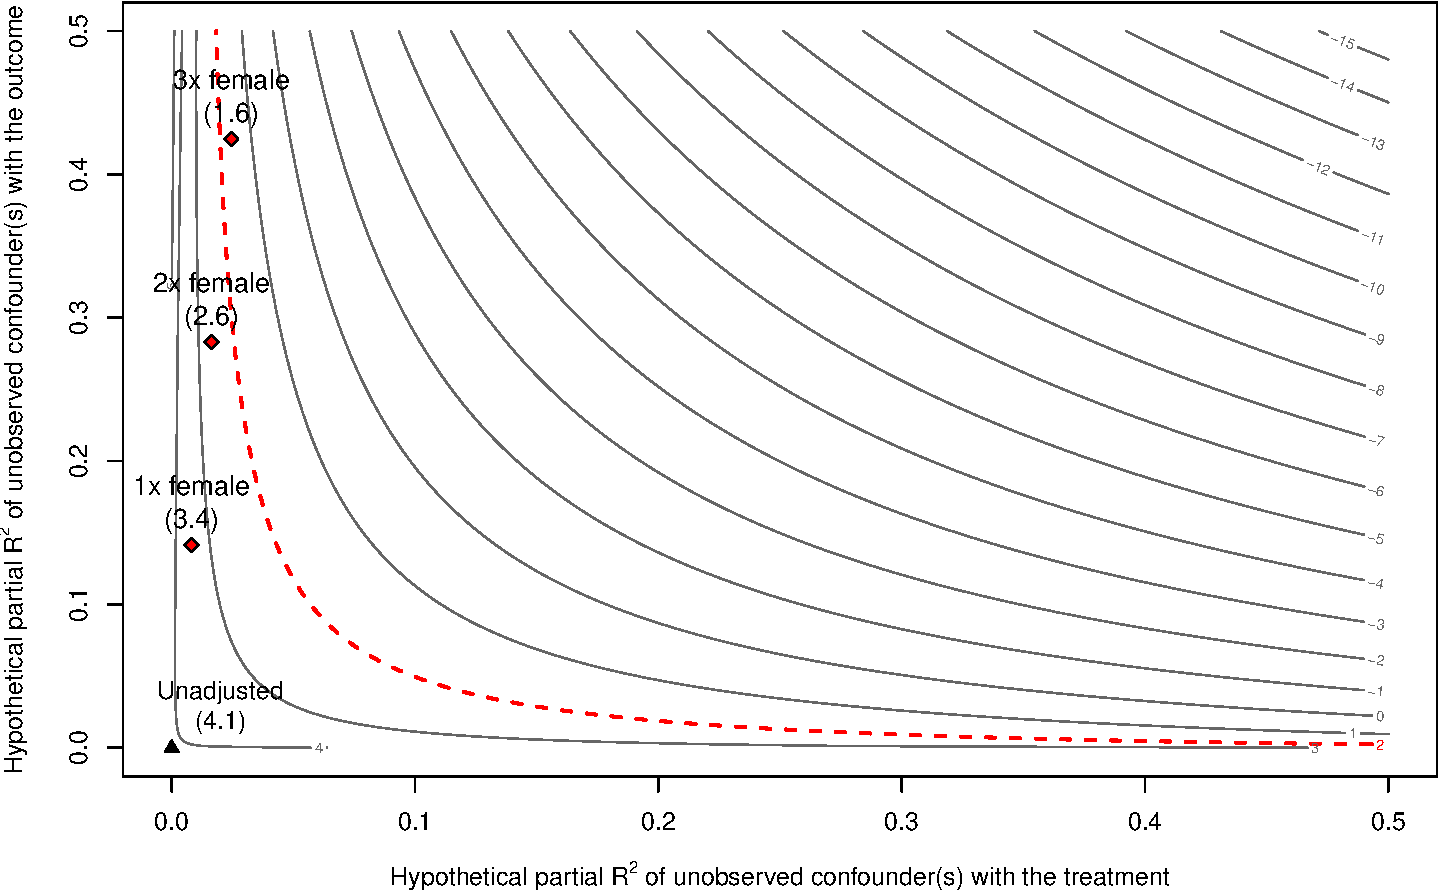
\includegraphics[width=\textwidth]{tcontour.pdf}\\[3pt]
\onslide<2->\scriptsize $t$ stays significant against a confounder up to ${\sim}2\times$ \textit{female}; loses significance by $3\times$.
\end{column}
\begin{column}{0.5\textwidth}
\centering
\onslide<3-> \textbf{Extreme scenario}\\[2pt]
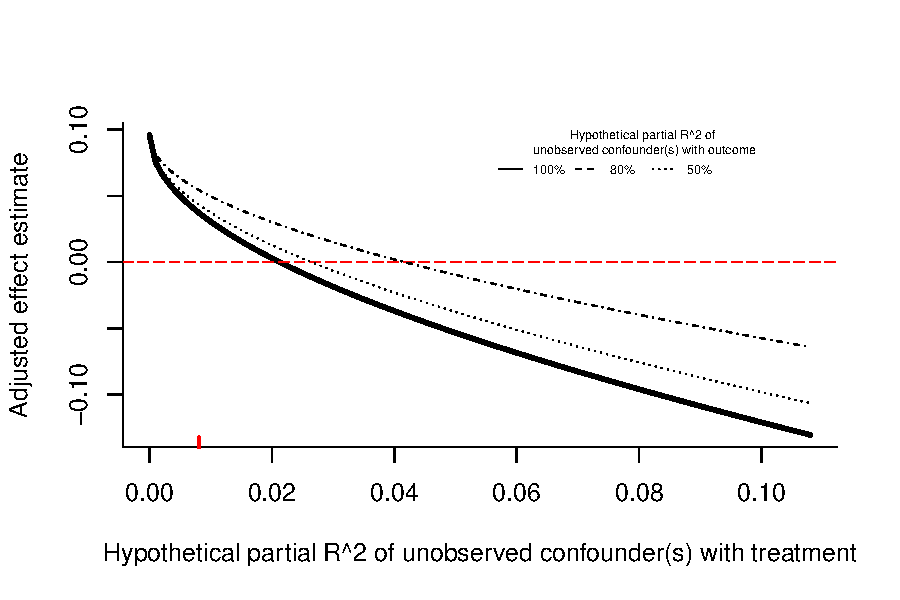
\includegraphics[width=\textwidth]{extreme_darfur.pdf}\\[3pt]
\onslide<4->\scriptsize Assume confounding explains \emph{all} residual outcome variance ($R^2_{Y\sim Z \mid \X, D} = 1$). $Z$ still needs to explain $\geq 2.2\%$ of $D$ to zero the effect. You pay a real price when you can't bound.
\end{column}
\end{columns}
\end{frame}


%======================================================================
\section{Practice}
%======================================================================

\begin{frame}{How to argue it (and what readers should demand)}
\small
\onslide<1-> \textbf{Defending a result.} Sometimes you can argue from design and context, e.g.\ for Darfur:\\
\scriptsize
\begin{quote}
``\dots aircraft dropped makeshift and unguided bombs over villages, and militia raided without concern for who they would attack --- the only known major exception, due to sexual assaults, was targeting gender, which is also one of the most visually apparent characteristics. \textbf{A confounder twice as strong as \textit{female} would be surprising.}''
\end{quote}
\small
Other times you can't, and the analysis simply reveals that, which is useful.\\

\bigskip
\onslide<2-> \textbf{Critiquing a result.} Dismissing a finding requires arguing for confounding of a specific strength, not just any confounder. ($t$ and df alone get you started; as a reader/reviewer you have the info.)\\

\bigskip

\onslide<3-> \textbf{The reframe.} This is never ``how much confounding is there'' --- it's ``how much would it take to overturn the conclusion.'' No magic RV threshold; the point is to refine the debate, not hide behind a number. Whether the answer is reassuring or unsettling, it's the honest conversation.
\end{frame}


\begin{frame}{Resources}
\small
\textbf{Papers} (all linked from \href{https://chadhazlett.com/publications.html}{chadhazlett.com/publications}):
\begin{itemize}
\item Cinelli \& Hazlett (2020). \emph{Making sense of sensitivity: Extending omitted variable bias.} JRSS B. --- the framework
\item Hazlett \& Parente (2023). \emph{From ``Is it unconfounded?'' to ``How much confounding would it take?''} JoP. --- applied / how-to-argue companion
\item Cinelli, Ferwerda \& Hazlett (2024). \emph{sensemakr: Sensitivity Analysis Tools for OLS in R and Stata.} Observational Studies. --- software paper
\item \emph{Wildfire Exposure Increases Pro-Climate Political Behaviors} --- worked applied example
\end{itemize}
\medskip
\textbf{Software \& tutorials}:
\begin{itemize}
\item \texttt{sensemakr} R/Stata + worked vignettes: \href{http://carloscinelli.com/sensemakr/}{carloscinelli.com/sensemakr}
\item Carlos Cinelli's site (talks, tutorials, videos): \href{http://carloscinelli.com}{carloscinelli.com}
\end{itemize}
\end{frame}

\end{document}


%======================================================================
\appendix
%======================================================================

\section{Appendix: matched-pair $\Gamma$ bounds}

\begin{frame}{Rosenbaum's $\Gamma$ for matched pairs}
\small
\begin{itemize}
\item<1-> A different sensitivity tradition (Rosenbaum 2002), with a single parameter $\Gamma \geq 1$ for departure from zero confounding.
\smallskip
\item<2-> Consider matched pairs $i, j$ with $X_i = X_j$. Under SOO, both have the same $\pi(X)$.
\smallskip
\item<3-> A binary unobserved $U$ may make their odds of treatment differ:
\[
\frac{1}{\Gamma} \;\leq\; \frac{\pi_i(1-\pi_j)}{(1-\pi_i)\pi_j} \;\leq\; \Gamma.
\]
\end{itemize}
\end{frame}


\begin{frame}{Formal sensitivity tests ($\Gamma$)}
\small
\begin{itemize}
\item<1-> $\Gamma = 1$: no hidden bias. $\Gamma = 2$: unit $i$ has twice the odds of treatment as $j$ despite identical $X$.
\smallskip
\item<2-> ``Primal'' version: only the odds of \emph{treatment} are varied; effect of $U$ on the outcome is taken to be infinite (worst-case).
\smallskip
\item<3-> At any chosen $\Gamma$, run a permutation-style test where assignment odds respect $\Gamma$.
\smallskip
\item<4-> Try increasing $\Gamma$ until significance is lost or the sign flips.
\smallskip
\item<5-> R: \texttt{psens()}, \texttt{hlsens()} in \texttt{rbounds}.
\end{itemize}
\end{frame}


\begin{frame}{Rosenbaum-style sensitivity: smoking example}
\begin{figure}
\centering
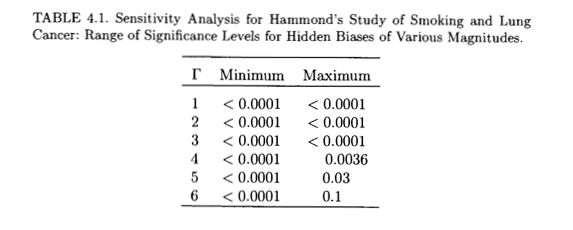
\includegraphics[scale=.6]{smoking_sensitivity.png}
\end{figure}
\onslide<2-> If a hidden confounder gave the unit with the worse outcome 6$\times$ higher odds of smoking, the adjusted estimate would lose significance.
\end{frame}


\section{Appendix: parametric (Imbens 2003)}

\begin{frame}{Imbens (2003): parametric approach}
\footnotesize
\begin{itemize}
\item Highly parametric:
\begin{itemize}\smallskip
\item Assume $Y_1, Y_0 \indep D \mid X, U$ with $U \sim \text{Bernoulli}(0.5)$, $U \perp X$.\smallskip
\item Logistic propensity: $P(D=1 \mid X, U) = \dfrac{\exp(X\theta + \gamma U)}{1 + \exp(X\theta + \gamma U)}$. $\gamma$ governs $U$--$D$ strength.\smallskip
\item Outcome conditionally normal: $Y \mid X, U \sim N(\alpha D + X\beta + \delta U,\ \sigma^2)$. $\delta$ governs $U$--$Y$ strength.\smallskip
\item Choose $(\gamma, \delta)$, find the MLE for $\hat{\alpha}(\gamma, \delta)$.
\end{itemize}
\item Reparameterize $(\gamma, \delta)$ as partial $R^2$'s with $D$ and with $Y$ for interpretability.
\end{itemize}
\bigskip
Trades stronger assumptions for more direct probabilistic interpretation. Carnegie--Dorie--Hill (2016) extends with BART for $\mu_0(X)$.
\end{frame}


\end{document}
